We followed the standard evaluation procedure for the WebQuestions dataset and used the original 70-30\% train-test split (3,778 training and 2,032 test instances), and F1-score as the evaluation metric:
$$f1(a^*, a) = 2\frac{precision(a^*,a) recall(a^*,a)}{precision(a^*,a) + recall(a^*,a)}$$
where $precision(a^*, a)=\frac{|a^* \cap a|}{|a|}$ and $recall(a^*, a) = \frac{|a^* \cap a|}{|a^*|}$, $a^*$ and $a$ are correct and given answers, which can be lists of entities.

We also report average precision and recall, as well as an F1 score of average precision and recall.
The results of existing approaches, our baseline and Text2KB systems is presented in Table \ref{table:webquestions_results}.
Modern search engines are very complex and usually include special components to deal with issues, similar to those described in this work, \eg entity identification.
Therefore, to demonstrate that the improvements of Text2KB doesn't simply come from using a commercial search engine, we include a variation of our system that uses Lucene search engine over english Wikipedia.

\begin{table*}
\caption{Performance of the Text2KB system on WebQuestions dataset compared to the existing approaches. The difference from the baseline Aqqu system is significant with p-value < 0.01}
\label{table:webquestions_results}
\begin{minipage}{17cm}
\centering
\begin{tabular}{| p{6cm} | p{1.5cm} | p{1.5cm} | p{1.5cm} | p{1.5cm} | }
\hline
System & avg Recall & avg Precision & F1 of avg P and R & avg F1 \\
\hline
OpenQA \cite{Fader:2014:OQA:2623330.2623677} & - & - & - & 0.35 \\
YodaQA \cite{baudivs2015systems} & - & - & - & 0.343\footnote{The reported score is F1@1. Text-based QA systems usually return a ranked list of answers and are evaluated either using ranking metrics or by taking the top candidate.} \\
\hline
SemPre \cite{Berant:EMNLP13} & 0.413 & 0.480 & 0.444 & 0.357\\
Subgraph Embeddings \cite{BordesCW14:emnlp} & - & - & 0.432 & 0.392\\
ParaSemPre \cite{berant2014semantic} & 0.466 & 0.405 & 0.433 & 0.399\\
Jacana \cite{yao2014information} & 0.458 & 0.517 & 0.486 & 0.330\\
Kitt AI \cite{yao-scratch-qa-naacl2015} & 0.545 & 0.526 & 0.535 & 0.443\\
AgendaIL \cite{berant2015imitation} & 0.557 & 0.505 & 0.530 & 0.497\\
STAGG \cite{yih2015semantic} & 0.607 & \textbf{0.528} & \textbf{0.565} & \textbf{0.525}\\
% STAGG (no duplicates\footnote{An answer of the STAGG system may contain duplicate entities, which are double counted by the evaluation script}) \cite{yih2015semantic} & 0.6067 & 0.5263 & 0.5634 & 0.5234 \\
\hline
Aqqu (baseline) \cite{ACCU:2015} & 0.604 & 0.498 & 0.546 & 0.494\\
Our system: Text2KB (Lucene + Wiki) & 0.632 & 0.498 & 0.557 & 0.514 \\
Our system: Text2KB (Bing + Web) & \textbf{0.635} & 0.506 & 0.563 & 0.522 \\
\hline
\end{tabular}
\end{minipage}
\vspace{-0.7cm}
\end{table*}

As we can see, Text2KB significantly improves over the baseline system and reaches the current best published result - STAGG \cite{yih2015semantic}, and we believe that this system will also benefit from the ideas of our work, and we will explore this question in Section \ref{section:analysis}.

\subsection{Ablation Study}

To study effects of different components in isolation we made a series of ablation studies.
For convenience, we introduce the following notations for different components of our system:

\begin{itemize}
\setlength\itemsep{-0.5em}
\item T - notable type score model as a ranking feature
\item DF - date range filter-based query template
% \item TF - using notable type based filter
\item E - using web search result snippets for question entity identification
\item W - using web search results for feature generation
\item CQA - using CQA-based \texttt{[question term, KB predicate]} PMI scores for feature generation
\item CW - features, computed from entity pairs language model, estimated on ClueWeb
\end{itemize}

In our results table we will use the notation \texttt{+$<$component$>$} to for a system with a certain component added, and \texttt{-$<$component$>$} when it is removed.
For example, the baseline system will be denoted as ``\texttt{Aqqu}''.
The same system with additional date range filter query templates and notable types score model is denoted as ``\texttt{Aqqu +DF+T}'', which represents the same system as ``\texttt{Text2KB -E-W-CQA-CL}''.
Our full system ``\texttt{Text2KB}'' can be also denoted as ``\texttt{Aqqu +DF+T+E+W+CQA+CL}''.

\begin{table}
\caption{Average Recall (R), Precision (Pr), and F1 of Aqqu (baseline), Text2KB (our system), and variations of TextKB with respective components removed. * indicates significant differences at p<0.05. }
\label{table:ablation:entities_vs_features}
\begin{tabular}{| p{4cm} | c | c | c | }
\hline
System & R & Pr & F1 \\
\hline
% THIS TELLS HOW MUCH EXTERNAL ENTITIES GIVE COMPARED TO MY OTHER IMPROVEMENTS
\texttt{Aqqu} (baseline) & 0.604 & 0.498 & 0.494\\
% baseline_typemodel_dates.log : baseline with types model +dates, but without any text-based data
% =\texttt{Aqqu +DF+T}
\texttt{Text2KB -E-W-CQA-CL} & 0.617 & 0.481 & 0.499 \\
% extent_dates_typemodel_rf100.log : -web-cqa-clueweb
\texttt{Text2KB -W-CQA-CL} & 0.627* & 0.492* & 0.508* \\  % AND FEATURES GIVE THE REST
% web_cqa_clueweb_typemodel_dates.log : -external entities (Text features on top my other improvements)
\texttt{Text2KB -E} & 0.634* & 0.497* & 0.514* \\  % AND FEATURES GIVE THE REST
%\hline
% extent_web_cqa_clueweb_dates_types_typemodel_rf100.log : everything, including type filters
%\texttt{Text2KB} & 0.6354* & 0.5059* & 0.5223* \\
\hline
\end{tabular}
\end{table}

First, let's see what are the improvements introduced by different components of our system (Table \ref{table:ablation:entities_vs_features}).
As we can see, additional date range filters and notable types model (\texttt{Text2KB -E-W-CQA-CL}) are responsible for an increased recall and a drop in precision compared to the baseline model.
Entity identification using web search results (\texttt{Text2KB -W-CQA-CL}) improves both precision and recall.
An even bigger improvement is achieved by introducing all additional text-based features, and since these improvements are independent, their combination boosts the performance even more.

Now, let's look into the relative importance of each of the data sources, we will remove or use a group of web search, cqa or clueweb-based features and see how the performance of the whole system changes (Table \ref{table:ablation:features}).

\begin{table}
\caption{Average Recall (R), Precision (Pr), and F1 of Text2KB variations with and without features based on web search results, CQA data and ClueWeb collection}
\label{table:ablation:features}
\centering
\begin{tabular}{| p{4cm} | c | c | c | }
\hline
System & R & Pr &  F1 \\
\hline
% THIS PART ANSWERS HOW GOOD ARE EACH OF THE PROPOSED DATASETS
% extent_cqa_clueweb_dates_typemodel_rf100.log : -web
\texttt{Text2KB -W} & 0.633 & 0.496 & 0.513 \\
% extent_web_clueweb_dates_typemodel_rf100.log : -cqa
\texttt{Text2KB -CQA} & 0.642 & 0.499 & 0.519 \\
% extent_web_cqa_dates_typemodel_rf100.log : -clueweb
\texttt{Text2KB -CL} & 0.644 & 0.505 & 0.523 \\
\hline
% extent_web_dates_typemodel_rf100.log : -clueweb-cqa
\texttt{Text2KB} (Web search only) & 0.642 & 0.503 & 0.522 \\
% extent_clue_dates_typemodel_rf100.log : -web-cqa
\texttt{Text2KB} (ClueWeb only) & 0.631 & 0.498 & 0.514 \\
% extent_cqa_dates_typemodel_rf100.log : -web-clueweb
\texttt{Text2KB} (CQA only) & 0.622 & 0.493 & 0.508 \\
%\hline
% extent_web_cqa_clueweb_dates_types_typemodel_rf100.log : everything, including type filters
%\texttt{Text2KB} & 0.6354 & 0.5059 & 0.5223 \\
\hline
\end{tabular}
\end{table}

As we can see, all data sources introduce an improvement to the baseline system, and web search results based features turned out to be the most useful.

% THIS EXPERIMENTS ARE REDUNDANT
%\begin{table}
%\caption{Evaluation study for our system with different text-based data sources used to generate features}
%\label{table:ablation:other}
%\begin{tabular}{| p{4cm} | c | c | c | }
%\hline
%System & avg Re & avg Pr &  avg F1 \\
%\hline
%AQQU & 0.604 & 0.498 & 0.494\\
%Text2KB -TF & 0.6429 & 0.5030 & 0.5220 \\
%\hline
% THIS PART SHOULD ANSWER HOW TEXT BASED FEATURED COMPARE TO EXTERNAL ENTITIES
% web_cqa_clueweb_typemodel_rf100.log : web+cqa+clueweb+typemodel -external-dates
%Text2KB +W+CQA+CW+T-E & 0.6351 & 0.4933 & 0.5104 \\
% web_cqa_clueweb_noext_rf100.log : web+cqa+clueweb -external-dates-typemodel
%Text2KB +W+CQA+CW-E & 0.6414 & 0.4981 & 0.5160 \\
% typemodel_rf100.log : type model only
%Text2KB +T-W-CQA-CL-E & 0.6131 & 0.4747 & 0.4918 \\
%\hline
%\end{tabular}
%\end{table}

\begin{figure*}
\centering
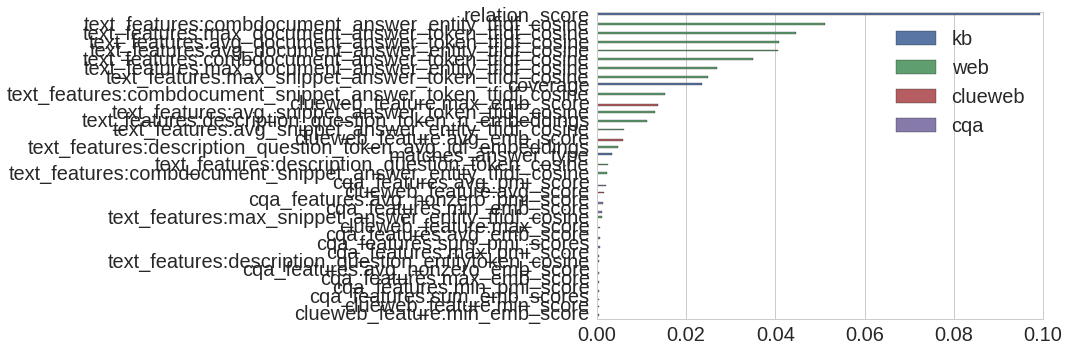
\includegraphics[width=0.8\textwidth]{img/feature_importances}
\caption{A plot of Gini importances of different features of our answer ranking random forest model (features marked * are not text-based and are provided for comparison)}
\label{fig:feature_importances}
\end{figure*}

Next, we will see which particular features are important in our random forest ranking model.
Figure \ref{fig:feature_importances} plots a subset of features ranked by their Gini index-based importance scores.
The figure supports the observation that web search results features are the most useful, however, other text data sources also contribute to the improvement.

In summary, Text2KB significantly outperforms the baseline system, and each of the introduced components contributes to this improvement.
Web search results data turned out to be the most useful resource, and it significantly improves the quality by helping with question entity identification and candidate ranking.
Next, we analyze the system performance in more detail, and investigate factors for future extension.